% - frame -----------------------------------------------------------------
\begin{frame}
   \frametitle{Příprava datasetu}
   \begin{columns}[t, onlytextwidth]
      \begin{column}[T]{0.5\textwidth}
         \begin{itemize}
            \item Nasbírání 100 fotek \emph{různých} telefonů
            \item Pro labelování použito \textbf{labelme} - časově náročné :(
            \item Převedení do jiného formánu vhodného pro trénování architektury \textbf{YOLOv5} za pomoci \textbf{RoboFlow}
            \item Rozšíření datasetu pomocí \textbf{augmentací}
         \end{itemize}
      \end{column}
      \begin{column}[T]{0.49\textwidth}
         \centering
         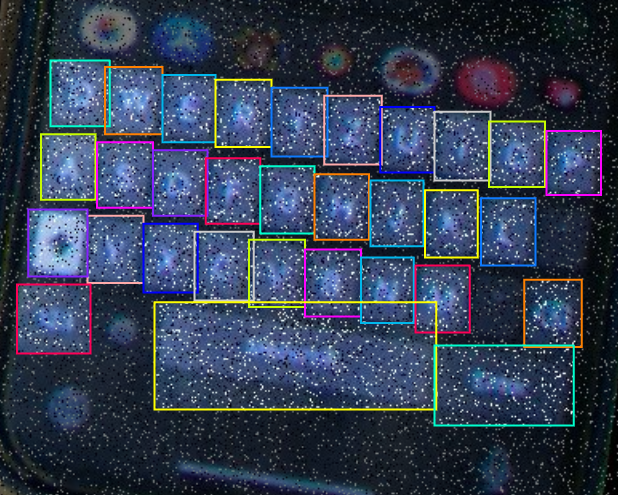
\includegraphics[width=0.8\linewidth]{labeling_demonstration.png}
      \end{column}
   \end{columns}
\end{frame}

% - frame -----------------------------------------------------------------
\begin{frame}
   \frametitle{Architektura a trénování}
   \begin{columns}[t, onlytextwidth]
      \begin{column}[T]{0.44\textwidth}
         \begin{itemize}
            \item Použita základní architektura \textbf{YOLOv5}, která umožnila detekovat více objektů najednou
            \parbox{\textwidth}{\tiny {\color{ctu4blue}Nelson J.}: \url{https://www.youtube.com/watch?v=MdF6x6ZmLAY}.}
% \parbox{\textwidth}{\tiny {\color{ctu4blue}Faigl J., Hollinger G.}: \textit{Unifying Multi-Goal Path Planning for Autonomous Data Collection}, {\color{ctu4blue}IROS}, 2014, 2937--2942.}
            \item Trénování proběhlo v \textbf{Google Colab}
            \item Nejlepších parametrů klasifikace bylo dosaženo s velmi \textbf{augmentovaným} datasetem a \textbf{1100} epochami
         \end{itemize}
      \end{column}
      \begin{column}[T]{0.55\textwidth}
         \centering
         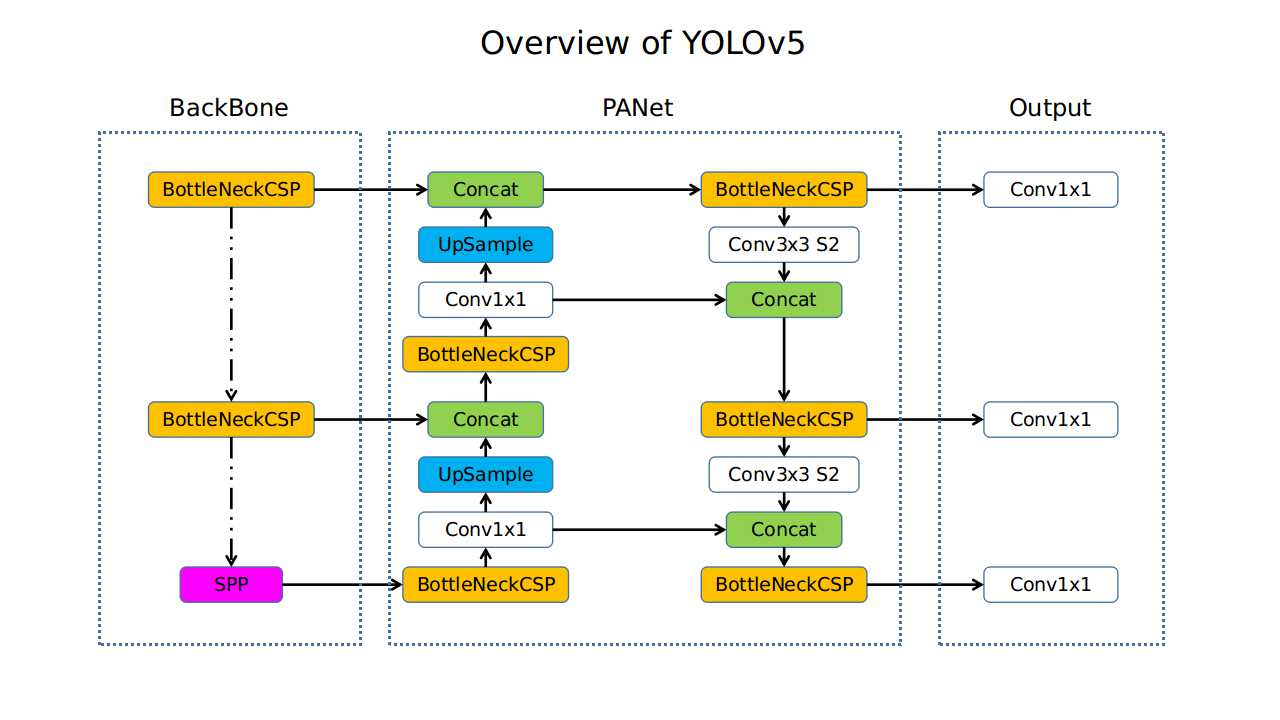
\includegraphics[width=\linewidth]{yolov5_arch.jpg}
      \end{column}
   \end{columns}
\end{frame}